\documentclass[10pt,a4paper,french]{article}
\usepackage[T1]{fontenc}
\usepackage[utf8]{inputenc}
\usepackage{fourier}

\usepackage[left=3.5cm, right=3.5cm, top=1.9cm, bottom=2.4cm]{geometry}

\usepackage{tikz}
\usetikzlibrary{arrows}

\usepackage{babel}
\DecimalMathComma

\definecolor{mygreen}{rgb}{0,0.4,0}
\definecolor{myviolet}{rgb}{0.5,0.5,1}
\definecolor{myblue}{rgb}{0,0,1}

\setlength\parindent{0mm}

#1: espacement entre les mini pages
#2: largeur pour l'image à droite
#3: texte à gauche
#4: "image" à droite
\newcommand\leftextrightim[4][2mm]{
	\begin{minipage}{\dimexpr\linewidth-#1-#2}
		#3
		
%		\vfill\null
	\end{minipage}
	\hfill
	\begin{minipage}{#2}
		#4
	\end{minipage}
}

\begin{document}


\subsection*{Exercice 1}

\leftextrightim{3cm}{
	Le périmètre d'un secteur de cercle de rayon $3 cm$ et $8 cm$. 

	Bla, bla, bla, bla, bla, bla, bla, bla, bla, bla, bla, bla, bla, bla, bla, bla, bla, bla, bla, bla, bla, bla, bla, bla, bla, bla, bla, bla, bla, bla, bla, bla, bla...

	Trouver l'aire de ce secteur.
}{
	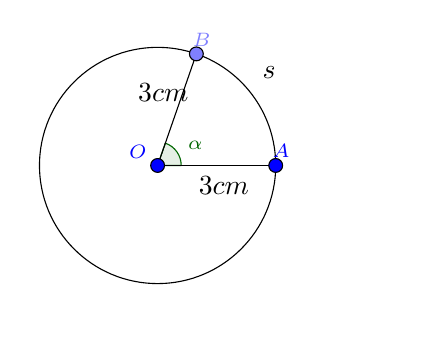
\begin{tikzpicture}[line cap=round,
	                    line join=round,
	                    >=triangle 45,
	                    x=.50cm, y=.50cm]
    \clip(-4.3,-3.08) rectangle (5.3,4.5);
    \draw [shift={(-1.,1.)},
           color=mygreen,
           fill=mygreen,
           fill opacity=0.1] 
          (0,0) -- (0.:0.6) arc (0.:70.83675422400157:0.6) -- cycle;
    \draw(-1.,1.) circle (1.5cm);
    \draw (-1.,1.)-- (2.,1.);
    \draw (-1.,1.)-- (-0.015217664611802961,3.8337614140762395);
    \draw (1.42,3.76) node[anchor=north west] {$s$};
    \draw (-0.2,0.96) node[anchor=north west] {$3 cm$};
    \draw (-1.74,3.32) node[anchor=north west] {$3 cm$};
    \begin{scriptsize}
    \draw [fill=myblue] (-1.,1.) circle (2.5pt);
    \draw[color=myblue] (-1.5,1.34) node {$O$};
    \draw [fill=myblue] (2.,1.) circle (2.5pt);
    \draw[color=myblue] (2.14,1.36) node {$A$};
    \draw [fill=myviolet] (-0.015217664611802961,3.8337614140762395) circle (2.5pt);
    \draw[color=myviolet] (0.12,4.2) node {$B$};
    \draw[color=mygreen] (-0.04,1.52) node {$\alpha$};
    \end{scriptsize}
    \end{tikzpicture}
}

Bla, bla, bla, bla, bla, bla, bla, bla, bla, bla, bla, bla, bla, bla, bla, bla, bla, bla, bla, bla, bla, bla, bla, bla, bla, bla, bla, bla, bla, bla, bla, bla, bla...

\leftextrightim[1cm]{3cm}{
Le périmètre d'un secteur de cercle de rayon $3 cm$ et $8 cm$. 

Bla, bla, bla, bla, bla, bla, bla, bla, bla, bla, bla, bla, bla, bla, bla, bla, bla, bla, bla, bla, bla, bla, bla, bla, bla, bla, bla, bla, bla, bla, bla, bla, bla...

Trouver l'aire de ce secteur.
}{
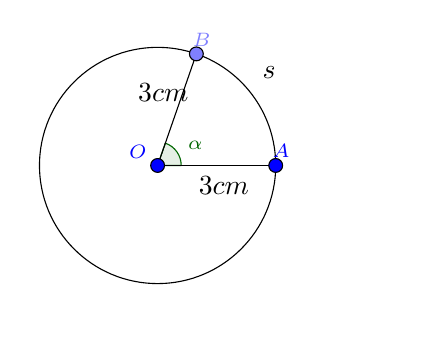
\begin{tikzpicture}[line cap=round,line join=round,>=triangle 45,x=.50cm,y=.50cm]
\clip(-4.3,-3.08) rectangle (5.3,4.5);
\draw [shift={(-1.,1.)},color=mygreen,fill=mygreen,fill opacity=0.1] (0,0) -- (0.:0.6) arc (0.:70.83675422400157:0.6) -- cycle;
\draw(-1.,1.) circle (1.5cm);
\draw (-1.,1.)-- (2.,1.);
\draw (-1.,1.)-- (-0.015217664611802961,3.8337614140762395);
\draw (1.42,3.76) node[anchor=north west] {$s$};
\draw (-0.2,0.96) node[anchor=north west] {$3 cm$};
\draw (-1.74,3.32) node[anchor=north west] {$3 cm$};
\begin{scriptsize}
\draw [fill=myblue] (-1.,1.) circle (2.5pt);
\draw[color=myblue] (-1.5,1.34) node {$O$};
\draw [fill=myblue] (2.,1.) circle (2.5pt);
\draw[color=myblue] (2.14,1.36) node {$A$};
\draw [fill=myviolet] (-0.015217664611802961,3.8337614140762395) circle (2.5pt);
\draw[color=myviolet] (0.12,4.2) node {$B$};
\draw[color=mygreen] (-0.04,1.52) node {$\alpha$};
\end{scriptsize}
\end{tikzpicture}
}


\end{document}
